\documentclass[12pt, a4paper]{scrartcl}
\usepackage [utf8] {inputenc} 
\usepackage [english,russian] {babel}
\usepackage{indentfirst}
\usepackage{misccorr}
\usepackage{graphicx}
\usepackage{amsmath}
\usepackage [warn] { mathtext }

\begin{document}
	\LARGE{\textbf{Федер Евгений, Домашнее задание №13}}\par
	
	%%%%%%%%%%%%%%%%%%%%%%%%%%
	\emph{\textbf{Задание 1.}}\par
	Давайте докажем от противного: пусть существуют пути $A$ и $B$ для которых $w(A) > w(B)$ и $B$ найден позже, чем $A$. Теперь рассмотрим 2 случая:
	\begin{enumerate}
	
	\item Они пересекаются по ребру, причем потоки идут в одну сторону. Тогда алгоритм опять бы взял $B$, а потом $A$.
	
	\item Они пересекаются по ребру и потоки идут в разные стороны. Рассмотрим 
	пример.\par
	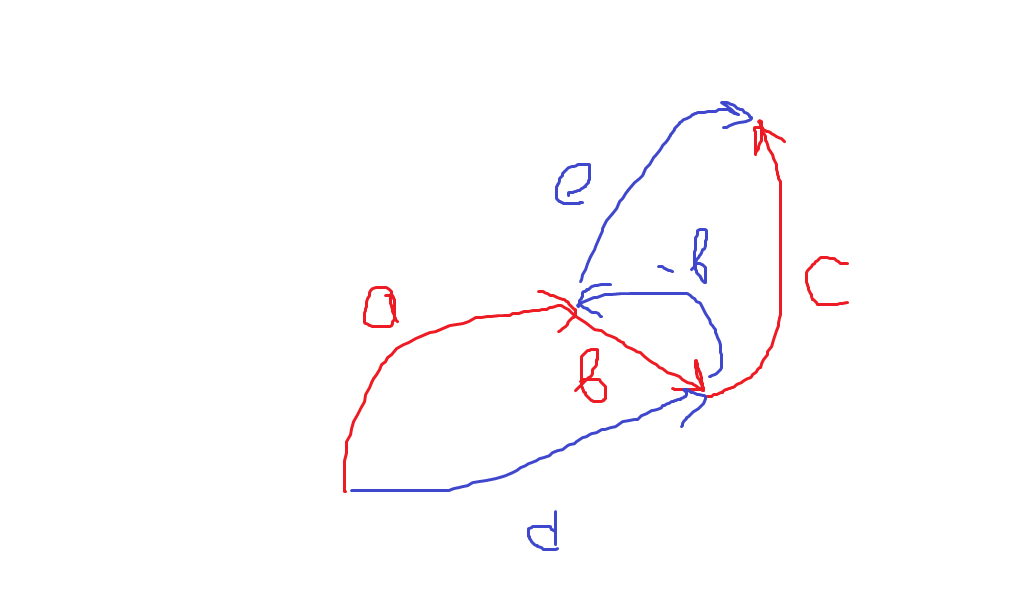
\includegraphics[scale=0.5]{ex1.png}\par
	Красный - А, синий - B.\par
	$w(A) > w(B) \Rightarrow a + b + c > d - b + e$ Но заметим, что так как мы сначала выбрали A, то\par
	$a + b < d$\par
	$b + c < e$\par
	Складывая 2 нижних и сравнивая с верзним получаем противоречие.
	\end{enumerate}
	Теперь давайте разобьем пути на кусочки, как выше(если их нет, то хорошо, мы бы выбрали B раньше чем А). И на каждом кусочке применим рассуждения выше(это будет верно, так как на кусочках минимализация веса должна сохраняться).
	
	%%%%%%%%%%%%%%%%%%%%%%%%%%
	\emph{\textbf{Задание 2.}}\par
	Наша задача эквивалентна нахождению макс потока мин стоимости из B в A и С. Преобразуем граф следующим образом. Каждому ребру G поставим стоимость - вес ребра, а вместимость - 1. Также добавим фиктивную вершину F, в которую проведем ребра из A и С весом 0 и вместимостью 1.\par 
	
	Теперь нам нужно найти вершинно простой путь. Для этого каждую вершину(кроме B и F) раздвоим и сделаем ребро из одной в другую вместимостью 
	1, и весом 0. Теперь все входящие ребра в вершину пусть входят в первую, а выходящие выходят из второй.\par
	
	Ищем максимальный поток мин стоимости из B в F. Если он не смог насытить оба ребра в F, то простого пути нет. Если насытил, то восстановим путь по массиву предков.\par
	Время - работа 2 Дейкстры, что с обычной кучей работает $О(ElogV)$
	
	%%%%%%%%%%%%%%%%%%%%%%%%%%
	\emph{\textbf{Задание 4.}}\par
	Построим полный двудольный граф с фейковыми вершинами S и T. Слева будут цвета шаров. Справа будут ящики. На каждом ребре из i в j вместимость будет 1, а стоимость - количества шаров i цвета, которые не лежат в j ящике. Из S в левую и из правой в T добавим ребра (1, 0).\par
	Теперь ищем max flow min cost(что значит найти совершенное паросочетание минимального веса). Итоговой стоимостью будет ответ, если поток насытит все ребра в T(оно насытит, так как у нас полный двудольный граф).
	Время работа - $О(V)$ Дейкстры за $О(V^2)$ - $О(V^3)$
\end{document}